\documentclass{arima-fr}
% force arXiv/HAL à compiler avec PDFLaTeX
\pdfoutput=1 

%%%%%%%%%%%%%%%%%%%%%%%%%%%%%%%%%%%%%%%%%%%%%%%%%%%%%%%
% Modules
\usepackage{array}
\usepackage{pgfplots}
\usepackage{graphicx}
\usepackage[utf8]{inputenc}
\usepackage[T1]{fontenc}
\usepackage{fancyhdr}
\pagestyle{fancy}
\usepackage{hyperref}
\usepackage[babel]{csquotes}

%%%%%%%%%%%%%%%%%%%%%%%%%%%%%%%%%%%%%%%%%%%%%%%%%%%%%%%
% En-tête
\title{Titre de l'article}
\author[1]{Eric BADOUEL}
\author[2]{Maurice TCHUENTE}
\author[*1,2]{Nabil GMATI}
\affil[1]{Affiliation 1, Pays A} 
\affil[2]{Affiliation 2, Pays B} 
% auteur correspondant avec son e-mail
\corrauthor{prénom.nom@mail.com}

%%%%%%%%%%%%%%%%%%%%%%%%%%%%%%%%%%%%%%%%%%%%%%%%%%%%%%%
%Code pour les citations de logiciels 
\usepackage[
  style=numeric-comp,
  datamodel=software, % extend the datamodel with entries for software
  abbreviate=false,
  natbib=true,
  sorting=ynt,
  backend=biber,
  bibencoding=utf8,
  giveninits=true,
  url=false,
  doi=false,
  defernumbers,
  maxcitenames=10,
  defernumbers=false,
  maxbibnames=100]{biblatex}
%
% Load the software biblatex style
%

\usepackage{software-biblatex}
%
% Set software specific bibliography options
%
\ExecuteBibliographyOptions{
  halid=true,
  swhid=true,
  swlabels=true,
  vcs=true,
  license=false}
%
% Make title an hyperlink to the DOI or URL to make the result leaner (suggested by N. Rougier 4/4/2020)
%

\newcommand{\doiorurl}{%
 \iffieldundef{doi}
    {\iffieldundef{url}
       {}
       {\strfield{url}}}
    {http://dx.doi.org/\strfield{doi}}%
}
\newcommand{\myhref}[1]{%
 \ifboolexpr{%
  test {\ifhyperref}
  and
  not test {\iftoggle{bbx:url}}
   and
   not test {\iftoggle{bbx:doi}}
  }
  {\href{\doiorurl}{#1}}
  {#1}%
}
\DeclareFieldFormat{title}{\myhref{\mkbibemph{#1}}}
\DeclareFieldFormat
  [article,inbook,incollection,inproceedings,patent,thesis,unpublished]
  {title}{\myhref{\mkbibquote{#1\isdot}}}
\addbibresource{ARIMA-FR.bib}



%%%%%%%%%%%%%%%%%%%%%%%%%%%%%%%%%%%%%%%%%%%%%%%%%%%%%%%
\pgfplotsset{compat=1.17}
\begin{document}
\maketitle





%%%%%%%%%%%%%%%%%%%%%%%%%%%%%%%%%%%%%%%%%%%%%%%%%%%%%%%
\abstract {

Sed non est ac erat varius mattis vestibulum tristique massa. Fusce leo elit, volutpat non massa nec, semper iaculis enim. Praesent commodo ante nec arcu dapibus dapibus commodo sit amet tellus. Donec auctor a ante non semper. Interdum et malesuada fames ac ante ipsum primis in faucibus. Nunc cursus dolor vitae massa fringilla semper. Ut nisl purus, porta id pretium tempus, porttitor sit amet felis. Maecenas nec leo faucibus, accumsan leo quis, rhoncus ante. Morbi a libero mollis, pellentesque tellus vel, consequat justo. Interdum et malesuada fames ac ante ipsum primis in faucibus.}

\keywords{Magna condimentum ; Vel ligula ; Elementum}





%%%%%%%%%%%%%%%%%%%%%%%%%%%%%%%%%%%%%%%%%%%%%%%%%%%%%%%
\section{Introduction}
Sed eu tempor ipsum, vel cursus arcu. Maecenas non dignissim nunc, ac ornare tortor. Aenean pretium arcu metus, id pulvinar enim tempus nec. Mauris faucibus mollis sodales.

Sed
porttitor sed metus vitae vestibulum. Quisque a vehicula nunc. Aenean fringilla condimentum diam, ac gravida quam. Integer ultrices feugiat enim nec tempus. Vestibulum ornare in magna ultrices dapibus. Nulla facilisi. 





%%%%%%%%%%%%%%%%%%%%%%%%%%%%%%%%%%%%%%%%%%%%%%%%%%%%%%%
\section{Section}
%%%%%%%%%%%%%%%%%%%%%%%%%%
\subsection{Sous-section 1}
Pellentesque dignissim ultrices fringilla. Vivamus eu luctus ante, vel bibendum magna. Curabitur elit purus, tincidunt non dui vitae, elementum bibendum neque. Curabitur ullamcorper sit amet justo at hendrerit. Fusce ut arcu imperdiet nibh mollis tempus a aliquet tellus. Quisque pharetra cursus nisi, vel lobortis ante consectetur et. Vivamus sed congue neque. Proin pellentesque risus nec dui consequat rutrum. Vestibulum nunc diam, placerat quis auctor vel, faucibus non justo. Etiam dictum purus neque. Phasellus imperdiet mauris ligula, eu laoreet nisi elementum ut. Sed sed porta massa. Aenean faucibus risus ultrices ornare porta. Quisque faucibus ante a tincidunt vestibulum. Lorem ipsum dolor sit amet, consectetur adipiscing elit.


%%%%%%%%%%%%%%%%%%%%%%%%%%
\subsection{Sous-section 2}
%%%
\subsubsection{Sous-sous-section}
Suspendisse vel dui nec felis molestie tincidunt. Vestibulum rutrum ligula lacus, ac molestie nulla fermentum ornare. Nulla non nunc euismod, porta lacus vestibulum, malesuada massa. Curabitur massa eros, rutrum sed lectus sed, volutpat semper metus. Mauris hendrerit aliquam commodo.  Vivamus fermentum tempus pellentesque. Maecenas a hendrerit urna. In elit ipsum, ultrices non dolor in, pulvinar porttitor lacus. Nunc euismod nibh quis odio condimentum, a feugiat massa rutrum. Nulla erat erat, adipiscing vitae lectus id, consectetur fermentum elit. Nunc eu est eu neque dapibus semper. Nam commodo urna dapibus, tincidunt turpis a, cursus sem. Vivamus venenatis adipiscing mollis. Cras fringilla sodales lobortis. Aliquam aliquet felis id est cursus auctor. Duis sodales tellus vulputate lectus egestas volutpat.





%%%%%%%%%%%%%%%%%%%%%%%%%%%%%%%%%%%%%%%%%%%%%%%%%%%%%%%
\section{Tableaux et Figures}
%%%%%%%%%%%%%%%%%%%%%%%%%%
\subsection{Tableaux}
Cf. Table~\ref{tab:example}.

\begin{table}
  \newcolumntype{+}{>{\global\let\currentrowstyle\relax}}
  \newcolumntype{^}{>{\currentrowstyle}}
  \newcommand{\rowstyle}[1]{\gdef\currentrowstyle{#1}%
    #1\ignorespaces
  }
  \centering
  \begin{tabular}{+>{\bfseries}l^c^c^c^c}
    \hline
    \rowstyle{\bfseries}
    & S-Longueur & S-Largeur & P-Longueur & P-Largeur\\
    Setosa & 5.006 & 3.428 & 1.462 & 0.246\\
    Versicolor & 5.936 & 2.77  & 4.26  & 1.326\\
    Verginica & 6.588 & 2.974 & 5.552 & 2.026\\
    \hline
  \end{tabular}
  \caption{Morbi malesuada diam at magna condimentum.}
  \label{tab:example}
\end{table}

\subsection{Figures}

Si possible, regrouper les figures dans un bloc. Utiliser des images d'une résolution au moins égale à 300 dpi. S'assurer que les légendes sont lisibles et en français. Voir par exemple : Figure~\ref{fig:example} (issue de \url{http://www.texample.net/tikz/examples/pgfplots/}). Le titre doit être terminé par un point.


%%%%%%%%%%%%%%%%%%%%%%%%%%
\begin{figure}
  \centering
  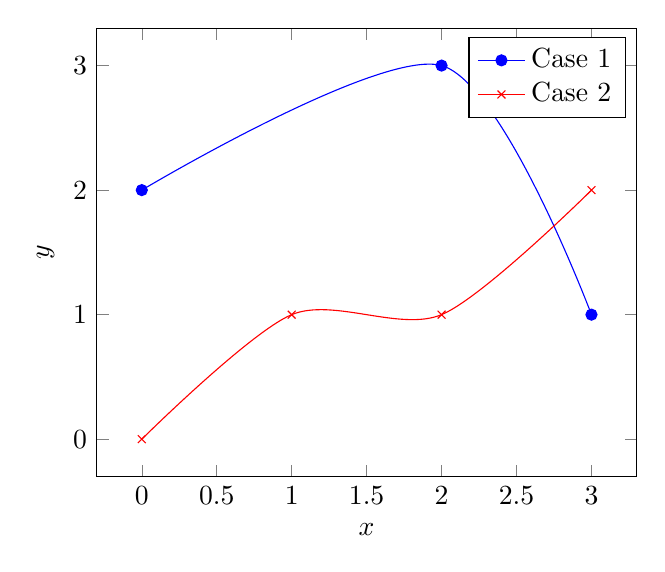
\begin{tikzpicture}
    \begin{axis}[
        xlabel=$x$,
        ylabel=$y$]
    \addplot[smooth,mark=*,blue] plot coordinates {
        (0,2)
        (2,3)
        (3,1)
    };
    \addlegendentry{Case 1}
    \addplot[smooth,color=red,mark=x]
        plot coordinates {
            (0,0)
            (1,1)
            (2,1)
            (3,2)
        };
    \addlegendentry{Case 2}
    \end{axis}
    \end{tikzpicture}
  \caption{figure de Christian Feuers\"anger; source: Pgfplots.}
  \label{fig:example}
\end{figure}

\begin{figure*}[ht] 
\resizebox{10cm}{9cm}
  {\includegraphics[width=11cm]{Lion.jpeg}}
  \centering
  \label{frog}
  \caption{Lion du Cameroun (crédit photo : Prénom Nom).}
  \end{figure*}
  




%%%%%%%%%%%%%%%%%%%%%%%%%%%%%%%%%%%%%%%%%%%%%%%%%%%%%%%
\section{Définitions, Algorithmes et Formules}
%%%%%%%%%%%%%%%%%%%%%%%%%%
\subsection{Définitions}
Pour les formules, utiliser le paquet \texttt{amsthm} et le style \texttt{arima} pour un formatage consistant.

\begin{definition}[alpha]
Curabitur ullamcorper sit amet justo at hendrerit.
\end{definition}

Puis, nous fixons la définition suivante.

\begin{definition}
Etiam sed nulla viverra, ultrices ligula ac, consectetur libero.
\end{definition}

Pour une liste, utiliser les "bullets" ou les tirets :
\begin{itemize}
  \item Nunc id justo scelerisque ;
  \item metus id enim iaculis tristique.
\end{itemize}


%%%%%%%%%%%%%%%%%%%%%%%%%%
\subsection{Formules}
Exemple de formule :
\begin{equation}
  Y=M.^tM-\beta.\langle M \rangle_l
\end{equation}

où $\langle M \rangle_l$ est le vecteur moyen d'une ligne de $M$. $\beta$ permet de réguler le taux de proches voisins.

Autre exemple de formule :
\begin{equation}
  K * N_c = Cst \pm 0.001\%
\end{equation}


%%%%%%%%%%%%%%%%%%%%%%%%%%
\subsection{Algorithmes}
Pour les algorithmes, utiliser la présentation de l'Algorithme~\ref{lst:example}. En cas de besoin, voir le paquet \texttt{listings}.

\begin{listing}
  \begin{lstlisting}
  partition(array, left, right)
     pivotIndex := choose-pivot(array, left, right)
     pivotValue := array[pivotIndex]
     swap array[pivotIndex] and array[right]
     storeIndex := left
     for i from left to right - 1
         if array[i] < pivotValue
             swap array[i] and array[storeIndex]
             storeIndex := storeIndex + 1
     swap array[storeIndex] and array[right]  // Move pivot to its final place
     return storeIndex
  \end{lstlisting}
  \caption{Fonction de partition d'un algorithme de tri.}
  \label{lst:example}
\end{listing}





%%%%%%%%%%%%%%%%%%%%%%%%%%%%%%%%%%%%%%%%%%%%%%%%%%%%%%%
\section{Conclusion et références}

%%%%%%%%%%%%%%%%%%%%%%%%%%
\subsection{Discussion}
Nam id eros massa. Fusce luctus purus a augue ullamcorper, sit amet vehicula mauris tristique. Suspendisse eget pulvinar odio, nec bibendum turpis. Nullam quis lectus porttitor, ullamcorper nisi et, condimentum leo. Quisque sed orci fermentum, rutrum velit eget, ultricies augue. Nunc porttitor consectetur tincidunt. Nulla tincidunt justo enim, vitae dignissim erat mattis ut. Nulla.


%%%%%%%%%%%%%%%%%%%%%%%%%%
\subsection{Conclusion}
Maecenas egestas metus id enim iaculis tristique. Etiam sed nulla viverra, ultrices ligula ac, consectetur libero. Nullam vitae massa ac odio pharetra condimentum. Maecenas in elementum libero, non gravida quam. Praesent adipiscing consectetur consectetur. Vivamus at orci sed augue varius hendrerit. Donec neque metus, dignissim nec erat at, ultricies consequat libero. Donec eget eleifend leo. Aliquam at nunc porta, mollis sapien eu, eleifend tortor. Nam egestas, metus ac pellentesque feugiat, lectus purus ornare est, vitae cursus felis turpis sit amet lacus. Donec consequat massa mi, ac suscipit arcu posuere et. Vivamus et semper risus. Sed ut arcu quam.


%%%%%%%%%%%%%%%%%%%%%%%%%%%%%%%%%%%%%%%%%%%%%%%%%%%%%%%
%Code pour bibliographie avec les logiciels 
\printbibheading
\printbibliography[heading=subbibliography,nottype=software,nottype=softwareversion,nottype=softwaremodule,nottype=codefragment,title={Publications}]
\printbibliography[heading=subbibliography,type=software,title={Software Project}]
\printbibliography[heading=subbibliography,type=softwareversion,title={Software versions, modules, excerpts and manuals}]
\nocite{*}


%%%%%%%%%%%%%%%%%%%%%%%%%%%%%%%%%%%%%%%%%%%%%%%%%%%%%%%
\appendix\footnotesize
%%%%%%%%%%%%%%%%%%%%%%%%%%%%%%%%%%%%%%%%%%%%%%%%%%%%%%%
\section{Annexe 1}
Dans Bibtex, comment écrire une citation d'un article de ARIMA (example: \citet{arima}) sans rien oublier et dans le bon format?
Voir la structure dans les commentaires à la fin de \textit{arima.tex}.





%%%%%%%%%%%%%%%%%%%%%%%%%%%%%%%%%%%%%%%%%%%%%%%%%%%%%%%
\section{Remerciements}
Nous tenons à remercier tous nos partenaires financiers : ANR ..., ERC ..., agences de financement, ...



%%%%%%%%%%%%%%%%%%%%%%%%%%%%%%%%%%%%%%%%%%%%%%%%%%%%%%%
\section{Biographie}
Il est possible ici d'insérer de courtes biographies des auteurs.





\end{document}